
\documentclass[nototal]{beamer}
\mode<presentation>
{
  \usetheme{Madrid}
 % \setbeamercovered{transparent}
}

\definecolor{sdsured}{RGB}{175,30,45}
\definecolor{asumaroon}{RGB}{153,0,51}
\definecolor{asugold}{RGB}{255,179,16}
\usecolortheme[named=asumaroon]{structure}
%\setbeamercolor{block title}{fg=asugold}
%\setbeamercolor{frametitle}{fg=asugold}
%\setbeamercolor{title}{fg=asugold}

\usepackage{verbatim}
\usepackage{fancyvrb}
\usepackage[english]{babel}
\usepackage[latin1]{inputenc}
\usepackage{times}
\usepackage{color}
\usepackage[T1]{fontenc}
\usepackage{graphicx} %sjr added
\graphicspath{{figures/}}
\usepackage{hyperref}

\author{Sergio Rey, Luc Anselin, David Folch}
\institute[ASU]{GeoDa Center for Geospatial Analysis and Computation\\School of Geographical Sciences and Urban Planning\\Arizona State University}
\title[PySAL -- GeoDaSpace]{Spatial Econometrics with PySAL and GeoDaSpace}
\subtitle{}
\date[RSAI 2010]{November 11, 2010}

% Delete this, if you do not want the table of contents to pop up at
% the beginning of each subsection:
 \AtBeginSubsection[]
 {
  \begin{frame}<beamer>
    \frametitle{Outline}
    \tableofcontents[currentsection,currentsubsection]
  \end{frame}
}


% If you wish to uncover everything in a step-wise fashion, uncomment
% the following command: 
\beamerdefaultoverlayspecification{<+->}
\begin{document}
\begin{frame}
  \titlepage
\end{frame}
\begin{frame}
  \frametitle{Outline}
  \tableofcontents[]
  % You might wish to add the option [pausesections]
\end{frame}



\section{} 


\section{} 


\section{} 

\section{GeoDa Center} 

\begin{frame}
	\frametitle{GeoDa Center for Geospatial Analysis and Computation}
  \begin{enumerate}
  \item Methods development
  \item Implementation through software tools
  \item Policy relevant research
  \item Dissemination through training and support
  \end{enumerate}
 \end{frame} 

\begin{frame}
	\frametitle{GeoDa Center}
 \begin{itemize}
 \item Arizona State University (beginning fourth year)
 \item Succeeds:
 \begin{itemize}
 \item Spatial Analysis Laboratory (UIUC)
 \item Regional Analysis Laboratory (SDSU)
 \end{itemize}
 \item Five core faculty
 \item Post-docs and graduate students
 \item Multi-disciplinary $\rightarrow$ geographers, computer scientists, economists
 \end{itemize}
 \end{frame} 

\begin{frame}
	\frametitle{Open Source vs. Free Software}
  All GeoDa Center software is free\dots \\ \qquad\qquad\qquad\qquad\qquad\dots some is also open source.
 
\begin{block}{Open Source}
 \begin{itemize}
 \item The raw code is supplied
 \item See how it works
 \item No black box
 \item Can be modified by the user
 \end{itemize}
 \end{block} 
\begin{block}{Free Software}
 \begin{itemize}
 \item No cost to use
 \item Black box
 \item GeoDa Legacy
 \end{itemize}
 \end{block} \end{frame} 

\begin{frame}
	\frametitle{Audience for GeoDa Center Tools}
 \begin{itemize}
 \item Interface
 \begin{itemize}
 \item Point-and-click
 \item Command line
 \end{itemize}
 \item Pedagogical
 \begin{itemize}
 \item Code as text
 \item Non-GIS experts
 \end{itemize}
 \item Audiences
 \begin{itemize}
 \item Social scientists: criminology, demography, urban studies, electoral studies, regional economics, \ldots
 \item Instructors
 \item Applied analysts: police, public health, agriculture, real estate, telco
 \end{itemize}
 \end{itemize}
 \end{frame} 

\begin{frame}
	\frametitle{Today}
 \begin{itemize}
 \item Overview and update of PySAL
 \item Spatial econometrics in PySAL and GeoDaSpace
 \end{itemize}
 \end{frame} 


\section{PySAL} 

\subsection{Background} 

\begin{frame}
	\frametitle{{\color{green}{Py}}thon {\color{green}{S}}patial {\color{green}{A}}nalysis {\color{green}{L}}ibrary}
 
\begin{block}{Leverage Existing Tools Development}
 \begin{itemize}
 \item GeoDa 
 \item STARS
 \item Others
 \end{itemize}
 \end{block} 
\begin{block}{Develop Core Library}
 \begin{itemize}
 \item Spatial data analytical functions 
 \item Enhanced specialization, modularization 
 \item Fill a void in Python libraries 
 \end{itemize}
 \end{block} 
\begin{block}{Flexible Delivery Mechanism}
 \begin{itemize}
 \item GUI, ArcGIS interface 
 \item Spatial analytical web services 
 \end{itemize}
 \end{block} \end{frame} 

\begin{frame}
	\frametitle{Philosophy}
 
\begin{block}{Pure Python}
 \begin{itemize}
 \item Code as text 
 \item Pedagogical goal 
 \end{itemize}
 \end{block} 
\begin{block}{Niche}
 \begin{itemize}
 \item Complementary 
 \item Evolutionary 
 \item Not revolutionary 
 \end{itemize}
 \end{block} \end{frame} 

\begin{frame}
	\frametitle{Functionality -- Big Picture}
  \begin{center}
  \includegraphics<1->[width=0.70\linewidth]{pysalGraphic.png}%
  \end{center}
 \end{frame} 

\subsection{Usage} 

\begin{frame}
	\frametitle{Regular Python Module}
 \VerbatimInput[frame=single,numbers=left,numbersep=3pt,
 fontsize=\small]{figures/pysalStart.txt}
 \end{frame} 

\begin{frame}
	\frametitle{File Input-Output}
 
\begin{block}{File Types}
 \begin{itemize}
 \item .shp $\rightarrow$ read, write
 \item .shx $\rightarrow$ read, write
 \item .dbf $\rightarrow$ read, write
 \item .gwt $\rightarrow$ read
 \item .gal $\rightarrow$ read
 \item .csv $\rightarrow$ read
 \item .wkt $\rightarrow$ read
 \item .geoda\_txt $\rightarrow$ read
 \end{itemize}
 \end{block} \end{frame} 

\begin{frame}
	\frametitle{File Input-Output -- Example (St. Louis Region)}
  \begin{center}
  \includegraphics<1->[width=0.80\linewidth]{stl.png}%
  \end{center}
 \end{frame} 

\begin{frame}
	\frametitle{File Input-Output -- Shapefile (.shp)}
 \VerbatimInput[frame=single,numbers=left,numbersep=3pt,
 fontsize=\small]{figures/pysalFileIO1.txt}
 \end{frame} 

\begin{frame}
	\frametitle{File Input-Output -- Shapefile (.dbf)}
 \VerbatimInput[frame=single,numbers=left,numbersep=3pt,
 fontsize=\small]{figures/pysalFileIO2.txt}
 \end{frame} 

\begin{frame}
	\frametitle{Spatial Weights (I)}
 \VerbatimInput[frame=single,numbers=left,numbersep=3pt,
 fontsize=\small]{figures/pysalWeights.txt}
 \end{frame} 

\begin{frame}
	\frametitle{Spatial Weights (II)}
 \VerbatimInput[frame=single,numbers=left,numbersep=3pt,
 fontsize=\small]{figures/pysalWeights2.txt}
 \end{frame} 



\section{Spatial Econometrics} 

\subsection{Background} 

\begin{frame}
	\frametitle{Spatial Econometric Tools}
 \begin{itemize}
 \item Not much commercially available
 \item Many specialized scripts
 \begin{itemize}
 \item Stata, SAS, SPSS, etc.
 \end{itemize}
 \item Toolboxs and libraries
 \begin{itemize}
 \item R: spdep, sphet
 \item MatLab: Econometrics Toolbox
 \end{itemize}
 \end{itemize}
 \end{frame} 

\begin{frame}
	\frametitle{Econometrics in Python -- Currently}
  \begin{quote}
  ``Since there is no free programming language that can be
  considered a \emph{lingua franca} of applied econometrics, choosing
  Python and writing or translating econometric routines may be
  worth the effort.''
  \end{quote}
  \qquad\qquad\qquad\qquad -- C. Choirat and R. Seri (2009), J. Appl. Econ.
 \end{frame} 

\begin{frame}
	\frametitle{Econometrics in Python -- Options}
 \begin{itemize}
 \item pyGauss
 \item pyTrix
 \item EconPy
 \item statsmodels / pandas
 \end{itemize}
 \end{frame} 

\begin{frame}
	\frametitle{Immediate Plan}
 \begin{itemize}
 \item OLS estimation with diagnostics for spatial effects
 \item 2SLS estimation with diagnostics for spatial effects
 \item Spatial 2SLS for spatial lag model (with endogeneity)
 \item GM and GMM estimation for spatial error model
 \item GMM spatial error with heteroskedasticity
 \item Spatial HAC estimation
 \end{itemize}
 \end{frame} 

\begin{frame}
	\frametitle{Challenges}
 \begin{itemize}
 \item Handle large problems
 \item Efficient spatial weights
 \item Modularity and reusability
 \end{itemize}
 \end{frame} 

\begin{frame}
	\frametitle{Functionality}
 \begin{itemize}
 \item Spatial weights creation
 \item Spatially lagged variable computation
 \item GMM estimation methods
 \item Diagnostics
 \item Allow endogeneity
 \end{itemize}
 \end{frame} 

\begin{frame}
	\frametitle{Delivery}
 \begin{itemize}
 \item Freestanding $\rightarrow$ GeoDaSpace
 \item Command line $\rightarrow$ PySAL
 \item ArcGIS toolbox
 \end{itemize}
 \end{frame} 

\subsection{PySAL} 

\begin{frame}
	\frametitle{PySAL Econometrics -- Setup OLS}
 \VerbatimInput[frame=single,numbers=left,numbersep=3pt,
 fontsize=\small]{figures/ols_commandLine.txt}
 \end{frame} 

\begin{frame}
	\frametitle{PySAL Econometrics -- Diagnostics Summary}
  \begin{center}
  \includegraphics<1->[width=0.53\linewidth]{ols_summary.png}%
  \end{center}
 \end{frame} 

\begin{frame}
	\frametitle{PySAL Econometrics -- Individual Diagnostics}
 \VerbatimInput[frame=single,numbers=left,numbersep=3pt,
 fontsize=\small]{figures/ols_diag.txt}
 \end{frame} 

\begin{frame}
	\frametitle{PySAL Econometrics -- Spatial Diagnostics}
 \VerbatimInput[frame=single,numbers=left,numbersep=3pt,
 fontsize=\small]{figures/spatial_diag.txt}
 \end{frame} 

\begin{frame}
	\frametitle{PySAL Econometrics -- Setup S2SLS}
 \VerbatimInput[frame=single,numbers=left,numbersep=3pt,
 fontsize=\small]{figures/s2sls_setup.txt}
 \end{frame} 

\begin{frame}
	\frametitle{PySAL Econometrics -- Setup GSLS (KP 1998, 1999)}
 \VerbatimInput[frame=single,numbers=left,numbersep=3pt,
 fontsize=\small]{figures/gsls_setup.txt}
 \end{frame} 

\subsection{GeoDaSpace} 

\begin{frame}
	\frametitle{Loosely Coupled Framework}
  \begin{center}
  \includegraphics<1->[width=0.70\linewidth]{software_links.png}%
  \end{center}
 \end{frame} 

\begin{frame}
	\frametitle{User Interface}
  \begin{center}
  \includegraphics<1->[width=0.60\linewidth]{space1.png}%
  \llap{\includegraphics<2->[width=0.60\linewidth]{space2.png}}%
  \llap{\includegraphics<3->[width=0.50\linewidth]{spaceW.png}}%
  \llap{\includegraphics<4->[width=0.60\linewidth]{space3.png}}%
  \llap{\includegraphics<5->[width=0.20\linewidth]{spaceL.png}}%
  \llap{\includegraphics<6->[width=0.60\linewidth]{space4.png}}%
  \llap{\includegraphics<6->[width=0.20\linewidth]{spaceL.png}}%
  \llap{\includegraphics<7->[width=0.60\linewidth]{space5.png}}%
  \llap{\includegraphics<8->[width=0.80\linewidth]{spaceR.png}}%
  \llap{\includegraphics<9->[width=0.60\linewidth]{space4.png}}%
  \end{center}
 \end{frame} 

\begin{frame}
	\frametitle{(Near) Future}
 \begin{itemize}
 \item Spatial regimes
 \item Probit (classic and spatial)
 \item Maximum Likelihood
 \item Panel data
 \end{itemize}
 \end{frame} 



\section{Conclusion} 

\subsection{Next Steps} 

\begin{frame}
	\frametitle{PySAL Release Schedule}
	\begin{block}{6 month release cycle}
 \begin{itemize}
 \item 1.0 - August 1, 2010
        \begin{itemize}
	  \item (700+ downloads since)
	\end{itemize}
 \item 1.1 - January 31, 2011
        \begin{itemize}
	  \item Spatial Dynamics
	  \item Space-Time Event Clustering
	  \item \alert{Spatial Econometrics}
	\end{itemize}
\item 2.0 - August 1, 2011
 \end{itemize}
 \end{block}
 \end{frame} 

\begin{frame}
	\frametitle{Other GeoDa Center Software}
 
\begin{block}{Currently Available}
 \begin{itemize}
 \item PySAL
 \item GeoDa (legacy)
 \item OpenGeoDa
 \item STARS
 \end{itemize}
 \end{block} 
\begin{block}{Coming Soon}
 \begin{itemize}
 \item GeoDaSpace
 \item GeoDaNet
 \item GeoDaWeight
 \item dynTM
 \end{itemize}
 \end{block} \end{frame} 

\begin{frame}
	\frametitle{Questions}
  \begin{center}
 \begin{figure}[htbp]
 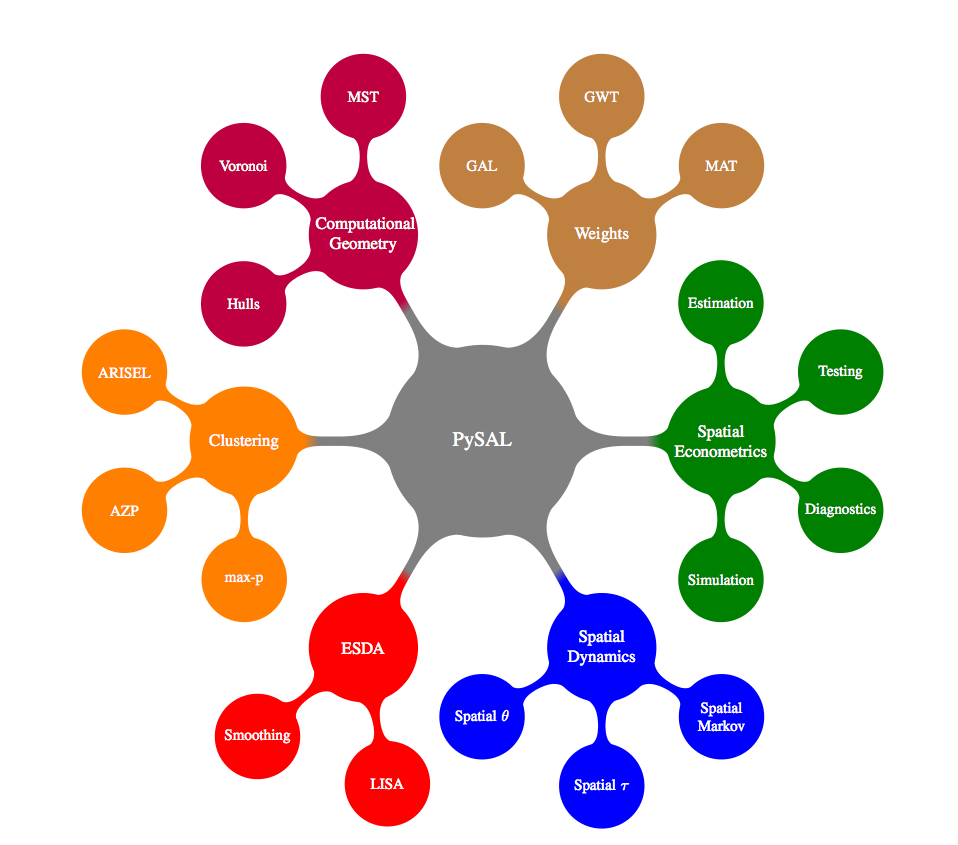
\includegraphics[width=0.60\linewidth]{pysalGraphic.png}
 \end{figure}
  {\color{blue}{\Large{geodacenter.asu.edu}}}\\
  {\color{blue}{\Large{www.pysal.org}}}
 \end{center}
 \end{frame} 




\section{} 


\section{}
\end{document}
